\chapter{Experimental Setup}
\label{ch:expsetup}

\epigraph{\emph{Ignore the glass ceiling and do your work. If you’re focusing on the glass ceiling,  focusing on what you don’t have, focusing on the limitations, then you will be limited.}}{Ava DuVernay}

another template

% The work in this thesis has been performed using data from the \ac{ATLAS} detector,  one of the particle detectors recording collisions of protons accelerated by the \ac{LHC} particle accelerator at \acs{CERN}. 
% In the following chapter, an introduction to the \ac{LHC} is given in section \ref{sec:ExpSetup:LHC}, followed by a discussion of the \ac{ATLAS} detector in section \ref{sec:ExpSetup:ATLAS}.  The discussion is focused on aspects important to the analyses of this thesis. 

% \section{LHC}
% \label{sec:ExpSetup:LHC}
% % \textcolor{red}{needs citations for accelerator chain, lumi clearing up between instantaneous and total, pileup formula. } 

% The \ac{LHC} \cite{LHCTDR,LHCMachine} is the largest particle accelerator in the world.  It is located at the \ac{CERN},  in Geneva,  Switzerland.  With its 27 km circumference, the accelerator ring is partially located in Switzerland and partially in France,  between 50-175 meters underground. 
% The \ac{LHC} was designed to accelerate protons in two separate beam pipes up to a centre of mass energy of 14 TeV.  It is also capable of accelerating heavy ions. 
% To keep the protons and heavy ions on the accelerator ring,  overall 9593 magnets are used.  These magnets include superconducting dipole and quadrupole magnets,  cooled down to 1.9 K (-271 $^{\circ}  C$).  The dipole magnets generate a magnetic field of 8.3 T. 

% \begin{figure}[htpb!]
% \centering
% \includegraphics[width=0.99\linewidth]{figures/ExpSetup/CernAcceleratorComplex2013.jpeg}
% \caption{Overview of the CERN accelerator facilities,  including the acceleration chain leading up to the \ac{LHC} \cite{CERNAcceleratorComplex2013} \label{fig:expSetup:acceleratorComplex}}
% \end{figure}

% Before the protons enter the \ac{LHC},  a chain of accelerators is used (see Fig.  \ref{fig:expSetup:acceleratorComplex}): starting from a hydrogen bottle,  negative hydrogen ions are fed into the Linear Accelerator 2 (LINAC2) and are accelerated up to 50 MeV.  Before getting inserted into the \ac{PSB} the ions are stripped of their electrons only leaving protons. The up to 2 GeV accelerated protons are then inserted into the Proton Synchrotron (PS),  followed by the \ac{SPS} which accelerates the protons from 60 GeV to 450 GeV before feeding the \ac{LHC}. Overall 8 radiofrequency cavities can push the energy of the protons in the LHC up to 14 TeV. 

% The \ac{LHC} so far provided proton and heavy ion beams for two data-taking periods.  Between 2009 and 2013 (known as Run-1), the LHC was operating with a centre-of-mass energy ($\sqrt{s}$) of 7 TeV and 8 TeV.  After a long shutdown (LS1) , the second run (Run-2) started in 2015 and ended in 2018,  providing 13 TeV collisions to the experiments around the \ac{LHC} ring.  In Figure \ref{fig:expSetup:acceleratorComplex} visualised yellow dots, there are four interaction points, housing the \acs{ALICE} \cite{ALICE},  \acs{LHCb} \cite{LHCb}, 
% \acs{CMS} \cite{CMS},  \acs{ATLAS} \cite{AtlasExperiment}, \acs{LHCf} \cite{LHCf} , \acs{TOTEM} \cite{TOTEM}, \acs{MoEDAL} \cite{MoEDAL} experiments,  among many other experiments.

% The instantaneous luminosity \cite{LHCMachine} is a measure of the accelerator:

% \begin{align}
% \mathcal{L} = \frac{N_b^ 2n_bf_{rev}\gamma_r}{4\pi\epsilon_n\beta^*}F
% \label{eq:theory:instantaneousLumi}
% \end{align}
% With $N_b$ the number of particles per bunch,  the bunches per beam $n_b$,  revolution frequency $f_{rev}$,  the relativistic gamma factor $\gamma_r$,   $\epsilon_n$ normalised transverse beam emittance as well as $\beta^*$, the beta function at the collision point,  determining the transverse spread of the particle beam.  The correction term F takes into account the beam crossing angle. 

% \begin{align}
% N_{event} = L_{int} \sigma_{event} = \sigma_{event} \int \mathcal{L} dt \label{eq:theory:integratedLumi}
% \end{align}

% A measure for the recorded data is the integrated luminosity over time, (see equation \eqref{eq:theory:integratedLumi}), connecting the luminosity with the number of events.  This can be seen for each month during Run-2 in Figure \ref{fig:expsetup:LumiOverview}.  This illustrates the overall 156 $\text{fb}^{-1}$ of a proton-proton collisions delivered to \ac{ATLAS} by the \ac{LHC} as well as the 139 $\text{fb}^{-1}$  of data collected by \ac{ATLAS} with detector conditions good enough to use the events in data analysis.

% \begin{figure}[htpb!]
% \centering
% \includegraphics[width=0.75\linewidth]{figures/ExpSetup/DeliveredRecordedLumi.png}
% \caption{Summary of the luminosity delivered by the LHC,  recorded by the ATLAS detector as well as the overall data good to use for physics analyses \cite{LumiPublicResultsPage} \label{fig:expsetup:LumiOverview}}
% \end{figure}

% As already hinted to in equation \eqref{eq:theory:instantaneousLumi},  protons in the acceleration chain are accelerated in so-called bunches to generate high instantaneous luminosity.  
% As a consequence,  many proton-proton interactions can happen during one crossing of bunches.  In Figure \ref{fig:expsetup:pileup},  the mean number of interactions per bunch crossing is given for all years of Run-2 data-taking. This so-called \textit{pile-up} reached above 70 number of interactions per bunch crossing in 2017.  
% \begin{figure}[htpb!]
% \centering
% 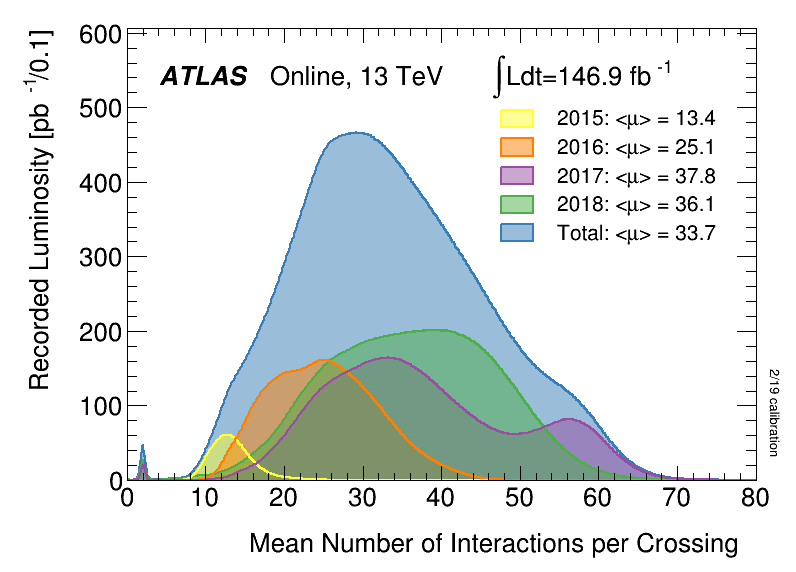
\includegraphics[width=0.75\linewidth]{figures/ExpSetup/PileupConditionsRun2.png}
% \caption{Pileup conditions throughout Run-2 \cite{LumiPublicResultsPage} \label{fig:expsetup:pileup}}
% \end{figure}

% %
% %\textcolor{gray}{
% %discuss accelerator chain - which energies in which accelerator 
% %some parts about magnet structure 
% %RF cavities for accelerations
% %include that the LHC is filled by single hydrogen bottle, its tilted to avoid water accumulating in the tunnel, magnet structure of the Lhc,  to focus beams and the RF cavities to accelerate.
% %}
% %.


% %include that the LHC is filled by single hydrogen bottle, its tilted to avoid water accumulating in the tunnel, magnet structure of the Lhc,  to focus beams and the RF cavities to accelerate.
% %Include some words on the bunch structure and the acceleration complex before the LHC. 
% %inlcude pileup discussion plot from lumi public results
% %integrated luminosity and instantaneous luminosity 
% %need to mention bunches, filling schemes to an extend, how often collisions are happening..
% %\textcolor{red}{have to mention what runs are - in connection with good runs lists}
% %\textcolor{red}{have to introduce run 1 and run 2 - because have run 1 analysis comparisons at some point? }
% %=====================================
% \FloatBarrier
% \section{ATLAS}
% \label{sec:ExpSetup:ATLAS}
% \FloatBarrier
% %=====================================
% The \ac{ATLAS} detector is located at Point 1 along the \ac{LHC}. This is the only \acs{CERN} site along the LHC ring with access to a main experiment, the \ac{SPS} as well as the LHC. 
% The overall structure is comparable to a barrel,  leading to the centre part of the detector being referred to as the barrel, as well as the large,  25m in diameter,  wheels on each side referred to as endcaps. 
% With its 25 meters tall and 44 meters length,  \ac{ATLAS} is the largest particle detector built on a collider so far. 
% It consists of multiple sub-systems and sub-detectors,  all built with different purposes in mind,  targeting momentum and energy reconstruction.  \ac{ATLAS} provides hermetic coverage around the beam axis,  enabling detection of all charged particles generated in the collisions in the plane orthogonal to the beam axis.  This is particularly important in searches for new physics, relying on analyses of momentum balances in the orthogonal plane such as discussed within this thesis.
% An illustration of the design of \ac{ATLAS} is given in Figure \ref{fig:expSetup:ATLASoverall}.  It is built up of multiple layers,  starting from the innermost component,  the \acf{ID},  providing tracking hits close to the beam pipe.  Surrounding the \ac{ID} is a system of two calorimeters. The outermost parts of \ac{ATLAS} are built by the muon spectrometer,  providing momentum reconstruction for muons passing through the inner detector layers. 
% Arguably one of the most striking features of \ac{ATLAS} is given through its magnet system.  Three superconducting Niobium-Titanium (NbTi) magnets span an overall length of 26m.  The first magnet system, the central solenoid,  is wrapped around the \ac{ID},  providing a 2 T axial magnetic field to curve the \ac{ID} tracks of charged particles. 
% The largest magnet parts are the eight barrel toroid coils,  intertwined with the outer muon system,  providing a total magnetic field of 4 T (0.5 T per coil) to measure the momentum of muons.  The toroid magnetic field is completed by the end-cap toroids,  also generating a magnetic field up to 4T for muons leaving \ac{ATLAS} close to the beam pipe. 

% \begin{figure}[htpb]
% \centering
% \includegraphics[width=0.9\linewidth]{../figures/ExpSetup/ATLAS_full.pdf} 
% \caption{Overview graphic of the ATLAS detector design \label{fig:expSetup:ATLASoverall},  with two people illustrated for scale reference \cite{ATLASfull}}
% \end{figure}

% Every component in \ac{ATLAS} working together enables the reconstruction and identification of a variety of particles with high precision.  An overview of the design capabilities of \ac{ATLAS} in terms of the momentum and energy resolution is given in Table \ref{tab:expSetup:Resolutions},  adapted from \cite{AtlasExperiment}.
% Here the resolution given lists first a stochastic term,  measuring the uncertainty based on the statistically dominated interaction of a particle with the material,  followed by a noise term,  which accounts for uncertainties due to electronic noise in the readout process. 

% \begin{table}[htpb!]
% \includegraphics[width=\linewidth]{figures/ExpSetup/ResolutionATLASDesign.pdf}
% \caption{Performance goals of the \ac{ATLAS} detectors' subsystems.  Units are given in GeV.  $\bigoplus$ indicating a sum in quadrature of the single terms for the total uncertainty \label{tab:expSetup:Resolutions}\cite{AtlasExperiment}. }
% \end{table}

% In the following, a brief overview of the detector is given; a more comprehensive description can be found in \cite{AtlasExperiment} as well as the Technical Design Reports of the subsystems,  as cited throughout the description below. 

% \subsection{ATLAS Coordinate system}
% The coordinate system used within \ac{ATLAS} is used throughout this thesis and shortly described in the following \cite{AtlasExperiment}. 
% The origin of the right-handed coordinate system is at the nominal interaction point,  with the positive x-axis pointing towards the centre of the \ac{LHC}.  The x-y plane is perpendicular to the beam axis,  defining the z-axis.  Towards the surface defines the positive y-axis.
% An azimuthal angle $\phi$ is defined around the beam axis, and a polar angle $\theta$ is the angle from the beam axis.  Instead of $\theta$ the rapidity $y$ is used for heavy objects:
% \begin{align}
% y = \frac{1}{2} \ln[(E+p_z)/(E-p_z)]
% \end{align}
% Differences in Rapidity are invariant under boosts along the beam axis.
% For massless objects or relativistic objects ($m << \vb*{p}$),  the pseudorapidity is used: 
% \begin{align}
% \eta = -\ln(\tan(\theta/2)) 
% \end{align}
% To quantify the distance between two objects,  $\Delta R$ is defined:
% \begin{align}
% \Delta R = \sqrt{\Delta\phi^2 + \Delta\eta^2} \label{eq:expsetup:deltaR}
% \end{align}
% The transverse momentum and energy are defined in the x-y plane,  with the transverse momentum given as $p_T = \sqrt{p_x^2 +p_y^2}$.

% %=====================================
% \subsection{Inner Detector}
% %=====================================
% A cross-section of the \ac{ID} system \cite{IDTDR} is shown in Figure \ref{fig:expSetup:InnerDetectors}, highlighting the distance of each subsystem from the beampipe. The innermost part of the \ac{ID}  is the \ac{IBL},  followed by three layers of pixel detectors.  At 299 mm radial distance from the beam pipe, four layers of \ac{SCT} modules are located before the \ac{TRT},  which extends the overall \ac{ID} detector size to a radius of 1082 mm.  The \ac{ID} allows for particle track reconstruction within $|\eta| < 2.5$.

% \begin{figure}[htpb!]
% \centering
% \subfloat[Sketch of the \ac{ID} and distances of its sub-detectors]{\includegraphics[width=0.49\linewidth]{figures/ExpSetup/ID_includingIBL.png}}
% \subfloat[Overview of barrel and end-cap \ac{ID} components, apart from \ac{IBL} \label{fig:expsetup:idendcaps}]{\includegraphics[width=0.49\linewidth]{figures/ExpSetup/ID_overview_noIBL.eps}}
% \caption{Slice view of the Inner Detector,  highlighting each sub-detectors distance to the beampipe \cite{IDsketchwithIBL} (a) and cut-out view of the barrel and endcap components,  not including the \ac{IBL} \cite{AtlasExperiment} (b).  \label{fig:expSetup:InnerDetectors}  }
% \end{figure}
% \paragraph{IBL - Insertable B-layer}
% After Run-1,  during a long shutdown in 2013-2014,  the pixel detector system was subject to maintenance and upgrades.  Within this set of upgrades,  %the \ac{DBM} was inserted within the pixel detector volume,  
% a 4th pixel layer at a 3.3 cm distance from a new,  smaller beam pipe (33 mm outer radius,  originally 36 mm).  A fourth pixel layer was a first in particle physics experiments \cite{IBLTDR,IBLproceedings} and has led to significant improvements in interaction vertex reconstruction and identification of b-hadron jets. 

% \paragraph{Pixel Detector}
% The innermost pixel layer,  the IBL,  is surrounded by three layers of pixel detectors,  arranged in barrels around the beam pipe \cite{PixelDesignPerformance,PixelPerformanceProceedings}.  The first layer is at a distance of 50.5 mm from the beam pipe's centre.  As can be seen in Figure \ref{fig:expsetup:idendcaps},  the end caps of the pixel layer consist of 3 disks around the beampipe,  stretching the length of the pixel component of the \ac{ID} to 1.4 m length along the beam axis.  The pixel detector consists of overall 1744 pixel modules with a nominal size of $50 \mu m x 400 \mu m$ in the $(\phi, z)$ plane ($\phi, r$ for the disk panels), comprising over 80 million readout channels.  
% The pixel and \ac{IBL} part of the ATLAS detector is crucial for tracking,  providing 4 pixel hits over the entire \ac{ID} pseudorapidity coverage ($|\eta| < 2.5.$).  
% %The resolution in the barrel is 10 mm (R-f) and 115 mm (z),as in the end-cap.

% \paragraph{Semiconductor Tracker}
% The pixel detector and \ac{IBL} are located within \ac{SCT} modules \cite{SCT}.  
% Similar to the pixel detector modules, the \ac{SCT} modules are semiconductor-based,  arranged into cylindrical layers around the beampipe in the barrel region,  forming disks in the endcap.  Since the \ac{SCT} modules only provide precise location along one axis,  two modules are combined back-to-back and rotated against each other to gain two dimensional spacial information.  Four layers are arranged in the barrel,  nine disks in each endcap side (see Fig. \ref{fig:expsetup:idendcaps}). Including the endcap disks, the \ac{SCT} extends up to $|z| < 2735 mm$. 

% \paragraph{Transition Radiation Tracker}
% The last part of the \ac{ID} is the \ac{TRT} \cite{TRTDesignPerformance},  in the barrel stretching from 554 mm to 1082 mm radial distance.  This detector is composed of 4 mm diameter straw tubes,  arranged in parallel to the beam pipe or radially in the barrel and end-cap, respectively.  Within $|\eta| < 2.0$,  three barrel rings and 18 end-cap units provide typically 36 hits per track. The straws are intertwined with polypropylene fibres for passing through particles to create transition radiation.  Inside the straws is a thin tungsten wire,  collecting charges drifting through the straws gas mixture (Xe, CO2 and O2). The level of radiation and collected charges in each straw can be used to discriminate between electrons and charged pions.  The \ac{TRT} only offers spatial information in the $(R-\phi)$ plane, no information in the z-direction can be extracted due to the straws orientation. 
 
% %70% Xe, 27% CO2 and 3% O2.
% %R − phi direction, while no information is provided
% %along the z-direction.
% %and can provide up to 36 hits per track.
% %up the TRT are straw tubes 4 mm in diameter,
% %with walls made of two multi-layer films, each 35  m thick.
% %The TRT is designed to provide a large number of hits, typically 36 per track,
% %with a coverage of j j < 2:0. It has an intrinsic accuracy of 130  m in R 􀀀  ,
% %providing no information in the z-direction
% %The TRT [71] consists of three barrel rings, with 32 modules each, and 18 end-caps units
% %31 2.2 The ATLAS detector
% %with 224 layers.
% %These are positioned
% %parallel to the beam pipe in the barrel and radial in the end caps. The
% %n the TRT this is done by polypropylene
% %fibres (foils), which are interwoven between the barrel (end-cap) straws, that enable
% %the production of transition radiation in the formof X-rays. The amount of radiation
% %produced can be used to distinguish between, e. g. electrons and charged pions, as the
% %amount of radiation would depend on how relativistic the charged particle is.

% %The TRT can discriminate between two signals, according to their
% %amplitude: the lowest charge is due to the minimum-ionising particles (MIPs) crossing the
% %gas, while the strongest signal is given by the transition-radiation photons absorbed in
% %the gas. This last class of events is originated by the electrons, hence the TRT is able to
% %contribute to electron identification on a straw-by-straw basis
% %\subsubsection*{SCT - Semiconductor Tracker }
% %\subsubsection*{TRT - Transition Radiation Tracker}
% %
% %gaseous/polypropylene-fibre transition radiation tracker (TRT) a
% %\subsubsection*{BCM - Beam Condition Monitor} --> beam condition monitor
% %\cite{BCM}
% %=====================================
% \subsection{Calorimeter System}
% %=====================================
% The overall \ac{ID} system is surrounded by two sets of calorimeters \cite{AtlasExperiment}.  An \acf{ECAL} \cite{LArTDR} in the inner most part, followed by a \ac{HCAL} \cite{TileTDR} (see Figure \ref{fig:expSetup:calorimeters}).  Both systems are designed to record the energy deposits of mainly electromagnetically interacting particles (electron,  photons) or the energy of hadrons,  based on hadronic interactions. 

% \begin{figure}[htpb!]
% \centering
% \includegraphics[width=0.75\linewidth]{figures/ExpSetup/Calorimeter_overview.eps}
% \caption{Illustration of the \ac{ATLAS} calorimeter system \cite{AtlasExperiment} \label{fig:expSetup:calorimeters}}
% \end{figure}

% Both calorimeters are so-called sampling calorimeters with alternating layers of absorber and active material.  The absorber layer triggers a shower development of consecutive interactions with the detector material,  the active layer is detecting the signal. The shower development and properties can be a helpful characteristic in particle identification.
% Overall,  the calorimeters cover the $|\eta|$ range below 4.9.  Two important quantities in connection with the calorimeters are the radiation length, $X_0$,  and the interaction length $\lambda$.   The radiation length  refers to the distance after which an electrons energy has been reduced to 1/e of its initial energy.  The interaction length describes the mean free path before the occurrence of an hadronic interaction.


% \paragraph{Liquid Argon Calorimeter}
% Liquid Argon (LAr) calorimeters \cite{LArTDR} are used in multiple parts of the calorimeter system.  First,  it is comprising the \ac{ECAL},  with two half barrels covering the central detector region, with a small (4 mm) gap at $z = 0$ and one end-cap on each side of the beamline (see Fig. \ref{fig:expSetup:ecal}).  Additionally,  the LAr technology is used for the hadronic calorimeters end-caps as well as a \ac{FCAL} ($3.1 < \eta < 4.9$). 
% The active material is LAr,  with copper and kapton electrodes for readout.  The absorber is made of lead with stainless steel sheets.  As can be seen in Figure \ref{fig:expSetup:ecal},  an accordion symmetry is used to ensure homogeneous coverage all over $\phi$.

% \begin{figure}[htpb!]
% \centering
% \subfloat[\label{fig:expSetup:ecal}]{\includegraphics[width=0.45\linewidth]{figures/ExpSetup/ECalVis.png}}
% \subfloat[\label{fig:expSetup:crack}]{\includegraphics[width=0.45\linewidth]{figures/ExpSetup/CrackRegionmaterial.png}}
% \caption{Visualisation of an \ac{ECAL} slice at $\eta = 0$ (a),   next to an overview of the material in terms of radiation lengths infront of the presampler and main \ac{ECAL} (b).  Both from \cite{AtlasExperiment}.}
% \end{figure}

% Infront of the \ac{ECAL} between $|\eta| < 1.52$ in the barrel region and $1.5 < |\eta| < 1.8$ in the end cap,  there is an additional layer of instrumented Liquid Argon,  the \textit{presampler}.  This is included in order to account for energy losses of particles before entering the \ac{ECAL}.  The first layer of the \ac{ECAL} has the finest granularity, comprising 4.3 $X_0$, followed by the second layer of 16 $X_0$ radiation lenghts in depth and a third layer with coarse granularity. 
% The total thickness in the barrel of the \ac{ECAL} is over 22 $X_0$,  over 24 $X_0$ in the endcap. 
% In Figure \ref{fig:expSetup:crack},  the amount of material infront of the presampler as well as the accordion part of the calorimeters is given in radiation lenghts.  Within the region of $ 1.37 < |\eta| < 1.52$,  a large amount of material is present.  This is due to the transition between the barrel and end-cap cryostats,  housing the calorimeters.  This region is knowns as the \textit{crack} region or transition region. 

% \paragraph{Tile Hadronic Calorimeter}
% The hadronic calorimeter is built of a tile calorimeter technology \cite{TileTDR} in the barrel and extend barrel region (between $0 < |\eta| < 1.7$,  see Figure \ref{fig:expSetup:calorimeters}).  Similar to the \ac{LAr} calorimeter the tile calorimeter is a sampling calorimeter,  with a steel absorber material as well as plastic scintillator tiles as active material.  The scintillator tiles are combined with optical fibres and photo-multipliers for signal readout.  In the barrel,  the tile calorimeter has an overall depth of roughly 9.7 interaction lengths. 

% %=====================================
% \subsection{Muon System}
% %=====================================
% The outermost part of the \ac{ATLAS} detector is the \ac{MS} \cite{MuonTDR}. It is embedded within the 4 T magnetic field generated by the barrel and endcap toroid magnets.  In Figure \ref{fig:expSetup:MS},  a quarter of the muon system is visualised, highlighting the different subsystems.  \acp{MDT} and \acp{RPC} form three layers around the barrel,  \acp{CSC} are used close to the beam pipe.  The \textit{Big Muon wheels},  forming the "lids" of the \ac{ATLAS} barrel structure,  are comprised of \ac{TGC} and \ac{MDT} subdetectors.  A short overview of the subsystems is given in the following.

% %d drift tube (MDT) and cathode strip (CSC) chambers for momentum determination an
% %resistive plate (RPC) and thin gap (TGC) chambers for triggering. The

% \begin{figure}[htpb!]
% \centering
% \includegraphics[width=0.8\linewidth]{figures/ExpSetup/MuonSpectrometer.png}
% \caption{Overview of a quarter of the muon spectrometer, showing all subsystems \cite{MuonTriggerPerformance} \label{fig:expSetup:MS}}
% \end{figure}

% \paragraph{MDT - Monitored Drift Tubes}
% The \ac{MDT} subdetectors of the muon spectrometer are drift tubes with a diameter of 29.97 mm.  They are filled with 93\% Ar,  7 \% CO2 and have a tungsten-rhenium wire in the middle.  There are in total 1171 \ac{MDT} chambers,  each layer with up to eight layers of drift tubes.  Overall 354240 tubes cover a pseudorapidity range up to $|\eta| < 2.7$,  providing high precision track coordinates perpendicular to the magnetic field.  In the innermost end-cap layer,  the \ac{MDT} chambers are replaced by \ac{CSC}'s. 

% %29.97 mm diameter drift tubes
% %93%Ar Å 7%CO2
% %tungsten-rhenium wire, measuring 50 ¹m in
% %Three to eight layers of drift tubes are used in
% %both barrel and end-caps to allow a total of twenty measurements for each track.\\
% %precision tracking
% %1171 MDT chambers, with a combined total of 354240 tubes.
% %ionisation
% %The coverage of the MDTs extends to
% %j j < 2:7 except in the innermost end-cap layer where they are limited to
% %j j < 2:0,
% %track coordinates
% %in the bending direction.
% %⌘| < 2.7.
% \paragraph{CSC - Cathode Strip Chamber}
% In the endcap in a pseudorapidity range of $2.0 < |\eta| < 2.7$,  the \ac{CSC} detectors provide a fast response and high spatial resolution,  similar to \ac{MDT}'s.  Since \ac{MDT} reach their maximum operational radiation tolerance close to the beampipe,  \ac{CSC} are used at the high radiation environment close to the beampipe.
% \ac{CSC} detectors are multiwire proportional chambers filled with the same gas mixture as \ac{MDT}'s.  They provide both $r$ and $\phi$ coordinates.
% %precision tracking
% %2:0 < j j < 2:7 replacing mdt's
% %incoming neutron
% %rate is expected to exceed 150 Hz=cm2, the maximum for safe operation of the
% %MDTs.
% %multiwire proportional chambers, using the same gas mixture
% %radial direction wire
% %characterised by a
% %fast response time and high spatial resolution
% %both radial and phi coordinate with
% Both \ac{MDT} and \ac{CSC} detectors are used for precision momentum measurements,  whereas \ac{RPC} and \ac{TGC} 
% detectors are used to provide fast information to the \ac{ATLAS} trigger system (see section \ref{sec:ExpSetup:trigger}).

% \paragraph{RPC - Resistive Plate Chambers}
% In combination with \ac{MDT}'s , \ac{RPC} detectors are used to provide a coarse,  quick,  secondary coordinate measurement.
% Each \ac{RPC} consists of two detector layers orthogonal to each other, providing $\phi$ and $\eta$ coordinate measurements.  The \ac{RPC} covers an overall pseudorapidity region up to $|\eta| < 1.05$.
% The detectors are named after the two resistive parallel plates of phenolic-melaminic plastic laminate within each chamber,  enclosing a gas mixture.
% %
% %triggering
% %provide a measure of the second coordinate in the
% %barrel.
% %They cover the pseudorapidity region |⌘| < 1.05.
% %much quicker response time compared
% %with the CSCs.
% %coarsely measure a second tracking coordinate in the
% %no-bending phi-projection to complement the
% %The chambers are filled with a gas mixture of C2H2F4 and a small fraction of resistive component
% %SF6 contained in two resistive parallel plates of bakelite, kept at a 2mm distance.
% %The two detector layers which form the chamber are placed orthogonally to read both the h and f
% %Two layers of chambers (middle station) provide the trigger for low-pT muons, while a
% %third one (outer station) is used for high pT trigger thresholds.

% \paragraph{TGC - Thin Gap Chambers}
% The last component of the \ac{MS} are \ac{TGC}.  They are multi-wire proportional chambers similar to \ac{CSC}'s,  but with a coarser granularity.  The gas filling is a mixture of CO2 and n-pentane (n-C5H12).  Similar to \ac{RPC} detectors,  \ac{TGC} are able to provide a signal faster than 25 ns,  allowing for a matchin of a signal to a specific bunch crossing.  Their fast readout time is used in the trigger system,  additional to \ac{MDT}, s they provide a secondary measurement of the azimuthal angle.   
% %triggering
% %TGCs are multi-wire
% %proportional chambers, filled with a mixture of CO2 and n-pentane (n-C5H12), and have a similar
% %structure as the CSCs but a higher granularity.
% %They are used as trigger chambers for muon tracks
% %and, in addition to the MDTs, they provide a second measurement of the azimuthal coordinate. Both
% %TGC and RPC chambers are designed to provide a signal over a time shorter than 25 ns.

% %=====================================
% %\subsection{Magnet System}
% %=====================================
% %\subsection{Forward Detectors}
% %%=====================================
% %%\subsubsection*{LUCID - Luminosity Cherenkov Integrating Detector}
% %%%\subsubsection*{AFP - ATLAS Forward Proton}
% %%\subsubsection*{ALFA - Absolute Luminosity For ATLAS}
% %%\subsubsection*{ZDC - Zero Degree Calorimeter}


% \FloatBarrier
% \subsection{The Trigger System}
% \label{sec:ExpSetup:trigger}
% %\subsubsection*{L1}
% %\subsubsection*{HLT}
% %\subsubsection*{MBTS - Minimum Bias Trigger Scintillator}

% With all the components of the ATLAS detector described above,  any interactions and electrical signals from the entire detector convolute into a large set of read-out information. Even without any proton-proton collisions provided by the \ac{LHC},  ATLAS can detect feedback from the detectors through for example cosmic muons. Storing every single interaction within ATLAS during collisions would exceed the storage capabilities of the CERN computing centres and simultaneous would not provide any differentiation between high energetic collision interactions and low energy scattering of the protons.
% The ATLAS trigger system has been designed to select collision events of interest to the multitude of physics analyses performed with ATLAS data.  To do so,  a two-stage trigger system was used during Run-2.  A visualisation of the trigger system, as well as the flow of data through this system, is given in Figure \ref{fig:expSetup:trigVis}.

% \begin{figure}[h]
% \centering
% \includegraphics[width=0.8\linewidth]{figures/ExpSetup/triggerSystem_withoutFTK.pdf}
% \caption{Overview of the ATLAS trigger system during Run-2.  Adapted from \cite{Run2TriggerOperation} \label{fig:expSetup:trigVis}}.
% \end{figure}

% The first trigger level is based in hardware.  This \textit{Level-1} trigger is built of processors digitizing the calorimeter readout and information from the muon spectrometers (\ac{TGC}, \ac{RPC}),  identifying electrons, photons,  tau leptons,  jets,  and can calculate missing transverse energy.  The L1Topo component of the Level-1 system allows for topological requirements such as invariant mass selections and distance measures to be taken into account in the Level-1 decision.  The final decision to keep or discard an event at Level-1 is made by the \ac{CTP}.  This Level-1 trigger step reduces the 40 MHz collision rate down to a maximum rate of 100 kHz \cite{Run2TriggerOperation} and passes on Regions-of-Interest in $\eta$ and $\phi$ to the next trigger step,  the \acf{HLT}.  Regions-of-Interest consist of neighbouring calorimeter cells in the \ac{ECAL} and \ac{HCAL},  a detailed discussion in connection with electron triggers is given in Chapter \ref{ch:trigger}.\\
% The \ac{HLT} is a software-based trigger,  a computing farm allowing for sequences of algorithms.  The \ac{HLT} is designed to reduce the event rate from 100 kHz to around 1 kHz that is saved.  The algorithms run on the \ac{HLT} farm have access to higher granularity calorimeter information as well as tracking information from the \ac{ID}.  A typical trigger sequence includes fast algorithms, designed to quickly reject events not targeted by the trigger,  followed by more precise algorithms that can run more time-consuming reconstruction and identification similar to events stored offline.  The exact sequence and type of algorithms considered at the \ac{HLT} are defined in the trigger \textit{menu}.  This comprises a database of triggers,  each trigger defining a sequence of algorithms and requirements on these algorithms for an event to pass the \ac{HLT}.  
% The overall set of triggers targeting various detector signatures associated with particles,  such as electrons,  muons or photons as well as missing transverse energy.  The trigger requirements are designed and budgeted in a way that the overall \ac{HLT} rate does not exceed 1 kHz. 
% In some cases,  even the reduction in event rate achieved through the \ac{HLT} algorithms for desired trigger requirements,  such as low momentum triggers,  is too high.  To keep the overall \ac{HLT} rate below 1 kHz in these cases,  triggers can still be included in the menu, but with a \textit{prescale}.  A prescale is an artificial scaling of the trigger,  only accepting every Nth trigger decision if the prescale factor is N.  This allows triggers with an otherwise high rate to still collect events.
% %\textcolor{red}{need to mention what trigger towers are}
% %\textcolor{red}{have mentioned the bandwidth and budgets of the different signatures? -- might have built up to this in the DAQ section}


